\subsection{R�ntgenr�hre}
F�r die Erzeugung von R�ntgenstrahlung kann eine R�ntgenr�hre verwendet. Eine schematische Darstellung einer R�ntgenr�hre ist ein Abb. \ref{fig:roehre} zu sehen.
Die R�ntgenr�hre besteht Haupts�chlich aus einer Gl�hwendel, einer Anode, und einer Vakuumglash�lle. Die Gl�hwendel wird zum emittieren von Elektronen verwendet. Mit einer Potentialdifferenz von 10 bis 100 kV werden die Elektronen zur Anode hin beschleunigt.
Die beschleunigten Elektronen treffen, auf die Anode, wo sie durch St��e R�ntgenstrahlen emittieren. Jedoch wird nur zu 1\% R�ntgenstrahlung erzeugt, der Rest geht in W�rme �ber, wodurch es n�tig wird die Anode zu k�hlen.

\begin{figure}[H]
	\centering
  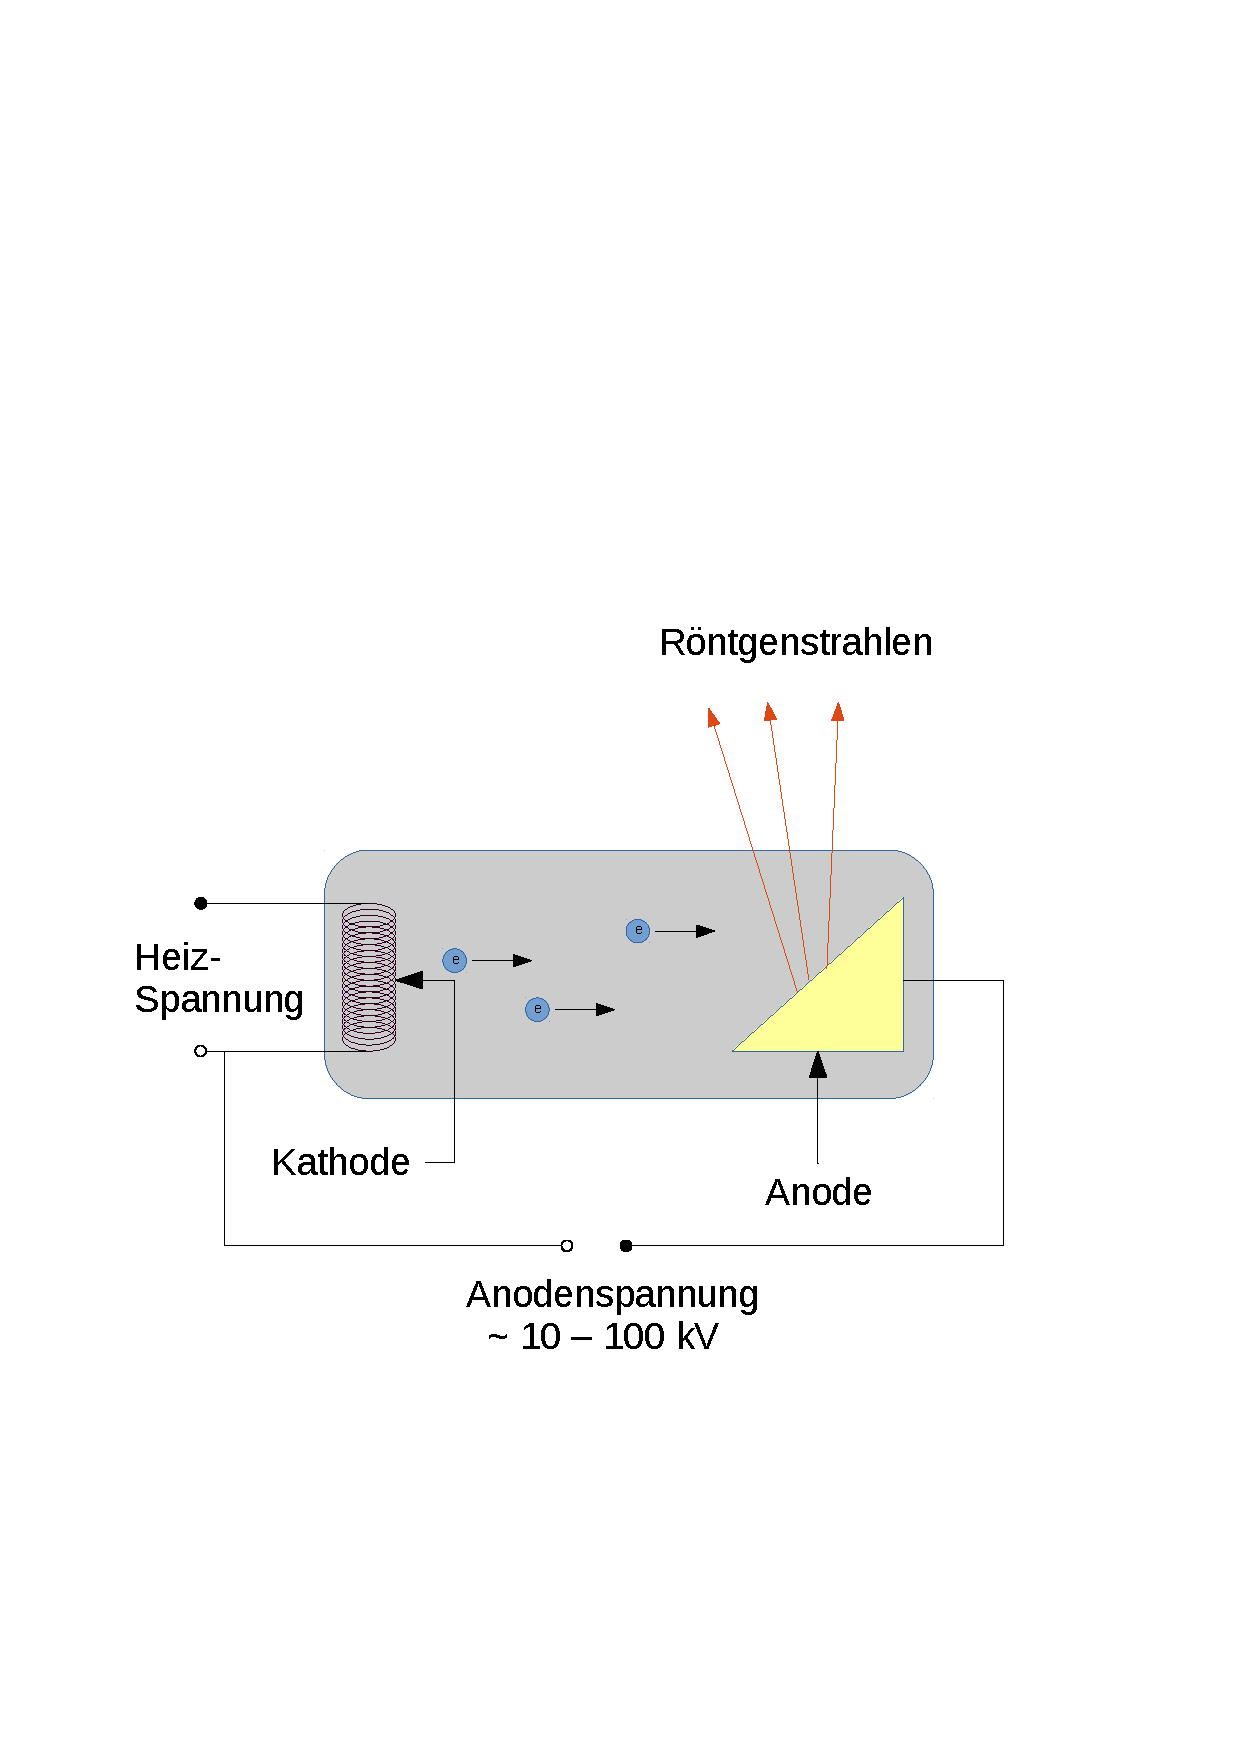
\includegraphics[trim = 20mm 60mm 20mm 100mm, clip, scale=1]{roehre.pdf}
	\caption{Schematischer Aufbau einer R�ntgenr�hre}
	\label{fig:roehre}
\end{figure}